\documentclass[twoside]{article}
\input{ISC18-english.sty}
	\usepackage{float}
%%%%%%%%%%%%%%%%%%%%%%%%%%%%  Make sure to compile twice for proper cross-references. %%%%%%%%%%%%%%%%%%%%%%%
%%%%%%% For proper display of references, compile the document twice. %%%%%%%%%%%%%%%%%%%%% 
%%%%%%%%%%%%%%% If using TeX Live, compile using pdflatex command %%%%%%%%%%%%%%%%%%%%%%%
\begin{document}

\thispagestyle{empty}
%%%%%%%%%%%%%%%%% Article title header  %%%%%%%%%%%%%%%%%%%%
\fancyhead[LE]{A Nonstandard Finite Difference Scheme for SPDEs}
%%%%%%%%%%%%%%%%% Article authors header   %%%%%%%%%%%%%%%%%%%%
\fancyhead[RO]{M. Namjoo, M. Aminian, and M.Karami }
\begin{center}
{
\includegraphics [height=25mm, width=150.3mm] {Images/isc18E}} \\
\vspace*{-1.8cm}
%\begin{center}
%\color{blue} 
%{\hspace{0.1cm}\rule{\textwidth}{1mm}}\\
%\end{center}
\vspace*{4cm}
%%%%%%%%%%%%%%%%% Article title  %%%%%%%%%%%%%%%%%%%%
{\Large \bf Construction and Analysis of a Nonstandard Finite Difference Scheme for Stochastic Partial Differential Equations}\\
%%%%%%%%%%%%%%%%% Article authors and affiliations %%%%%%%%%%%%%%%%%%%%
{\bf
Mehran Namjoo\footnote[1]{{\bf Corresponding Author:} {\tt namjoo@vru.ac.ir }}, Mehran Aminian$^2$, and Mehdi Karami$^3$   \\
$^{1,2,3}$Department of Mathematics, Vali-e-Asr University of Rafsanjan,
Rafsanjan, Iran.}
\end{center}
\rule{\textwidth}{0.2mm}\\
%%%%%%%%%%%%%%%%% Article abstract  %%%%%%%%%%%%%%%%%%%%
\noindent{\bf Abstract:}\\
This paper is devoted to the development and comprehensive analysis of a 
nonstandard finite difference (NSFD) scheme for It\^{o} stochastic partial 
differential equations (SPDEs). The qualitative properties of the proposed 
scheme, including consistency, stability, and convergence, are thoroughly 
investigated. Numerical simulations are presented to demonstrate the accuracy 
and computational efficiency of the proposed scheme.

 
\noindent{\bf Keywords:} 
Nonstandard finite difference scheme, consistency, stability, convergence, stochastic partial differential equations.
 \\
\noindent{\bf Mathematics Subject Classification (2010):} $\rm 65M06$, $\rm 65M12$, $\rm 60H15$.  \\
\hspace{1cm}\rule{\textwidth}{0.2mm}\\
%%%%%%%%%%%%%%

\section{Introduction}
\raggedbottom
\allowdisplaybreaks
Over the past few decades, stochastic partial differential equations (SPDEs)
have emerged as a powerful framework for modelling realistic phenomena, as
they accurately reflect the fundamentally random nature of the underlying
processes. SPDEs arise in a wide range of scientific disciplines, including
chemical physics, fluid mechanics, biology, and economics. Consequently, this
class of problems has attracted growing interest, and considerable research
effort has increasingly been devoted to the analysis of SPDEs. Moreover, since
the exact solutions of SPDEs are, in many cases, difficult or even impossible
to obtain, the development of effective numerical methods for their
approximation has become essential. Stochastic finite difference (SFD) schemes are among the most widely used numerical methods for approximating the solutions of SPDEs. The works \cite{Namjoo:etal:2024, Baleanu:etal:2023, Karami:etal:2023, Namjoo:Mohebbian:2016, Namjoo:Mohebbian:2019} are devoted to the convergence and stability analysis of several stochastic finite difference schemes for classes of SPDEs.
. This paper develops a novel NSFD scheme for SPDEs driven by a one-dimensional white noise process. The remainder of this paper proceeds as follows.  Section 2
briefly reviews the structure of NSFD schemes. Section 3 presents an
explicit NSFD scheme for approximating the solution of SPDEs. In
Section 4, the consistency, stability, and convergence of the
proposed NSFD scheme are established. Finally, Section 5 concludes the paper and presents some numerical results.


\section{Nonstandard Finite Difference Schemes for Initial Value Problems
}
In this section, we review the fundamental principles of NSFD schemes. Mickens introduced the NSFD framework for ordinary differential equations \cite{Mickens:2020}; this approach has been further employed by the authors in several studies~\cite{Namjoo:etal:2025, Namjoo:Zibaei:2019, Namjoo:etal:2018, Namjoo:Zibaei:2020, Karami:etal:2024}.
 To illustrate an NSFD scheme, we consider the following nonlinear initial value problem
\begin{equation*}
	\mathit{Y}^\prime(t)=f(\mathit{Y}(t)) ,\hspace{0.2in} \mathit{Y}(t_0)=\mathit{Y}_0,\hspace{0.2in}t\in[0,T_f].
\end{equation*} 
An NSFD scheme can be constructed by employing at least one of the following two steps. We utilize the discrete approximation
\begin{equation*}
	\mathit{Y}^\prime(t_k)\approx\frac{\mathit{Y}_{k+1}-\mathit{Y}_k}{\mathcal{X}(\Delta t)},
\end{equation*}
where $Y_k$ denotes the approximation of $Y(t_k)$ at time step $t_k = k\Delta t$ for $k = 0, 1, \ldots, N$. The nontrivial denominator function $\mathcal{X}(\Delta t)$ must be continuous and strictly increasing, satisfying the following criterion:
\begin{equation*}
	\mathcal{X}(\Delta t)=\Delta t+\mathrm{O}(\Delta t^2),\hspace{0.2in} 0<\mathcal{X}(\Delta t)<1, \hspace{0.2in} \Delta t\rightarrow 0.
\end{equation*}
Some examples of denominator functions are given in \cite{Namjoo:Zibaei:2020}:
$$
\frac{e^{\lambda\Delta t} - 1}{\lambda}, \quad \tanh(\Delta t), \quad \sin(\Delta t).
$$
Nonlocal approximations are applied to both nonlinear and linear terms; for example,
\begin{equation*}
	x(t)z(t)\rvert_{t=t_k}\approx x_{k+1}z_k,\hspace{0.2in}
	x(t)\rvert_{t=t_k}\approx x_{k+1},\hspace{0.2in}
	z^2(t)\rvert_{t=t_k}\approx z_kz_{k+1}.
\end{equation*}
\section{An explicit NSFD scheme for SPDEs}
In this section, we develop a nonstandard finite difference (NSFD) scheme
for solving the SPDE of the form
\begin{equation}\label{eq:spde}
	u_t(x,t)+a\gamma\, u_{xx}(x,t)+b\,u(x,t)+c\,u(x,t)\dot{W}(t)=0,
	\qquad x\in[0,1],\; t\in[0,1],
\end{equation}
subject to the initial and boundary conditions
\[
u(x,0)=u_0(x),\qquad u(0,t)=f(t),\qquad u(1,t)=g(t),
\]
where $b$ and $c$ are positive constants and $\dot{W}(t)$ denotes
white noise, modelled as a Gaussian process with zero mean \cite{Kloeden:Platen:1995}. The linear term of \eqref{eq:spde} is represented by the
nonlocal approximation
$u_k^n\approx\frac12\!\left(u_{k+1}^n+u_k^n\right),$ where $u_k^n$ denotes the
numerical solution at the grid point
$(x_k,t_n)=(k\Delta x,\,n\Delta t)$. The temporal and spatial derivatives,
together with the function $u(x,t)$ appearing in the deterministic part,
are discretized as
\[
u_t(k\Delta x,n\Delta t)\approx\frac{u_k^{n+1}-u_k^n}{\Delta t},\quad
u_{xx}\approx\frac{u_{k-1}^n-2u_k^n+u_{k+1}^n}{\Delta x^2},\quad
u_k^n\approx\frac{u_{k+1}^n+u_k^n}{2}.
\]
Substituting these approximations into \eqref{eq:spde} yields the explicit
NSFD scheme
\begin{equation}\label{eq:nsfd}
	u_k^{n+1}=-r\,u_{k-1}^n+(1+2r-s)\,u_k^n-(r+s)\,u_{k+1}^n-c\,u_k^n\,\Delta W_n,
\end{equation}
where $r=\frac{a\Delta t}{\Delta x^2}$, $s=\frac{b\Delta t}{2}$ and
$\Delta W_n=W\big((n+1)\Delta t\big)-W\big(n\Delta t\big)\sim N(0,\Delta t)$.
Throughout the remainder of this manuscript, the increments of the Wiener
process are assumed to be independent of the state $u_k^n$.

\section{On the Consistency, Convergence, and Stability of the Proposed NSFD Scheme}
Consider a SPDE of the form $Lu = G$ where $L$ denotes the differential operator and $G$ is source term. Let $L_h^n u_k^n = G_k^n$ denote the NSFD scheme. In order to analysis consistency and stability the NSFD scheme (3.2), it is very important to consider a norm. Hence, for a sequence $\{u_k^n\}_{0 \le k \le M}$, we define $||u^n|| = \sqrt{\sup_{0 \le k \le M} |u_k^n|^2}$. In order to get consistency, stability and convergence results, we give the following definitions \cite{Roth:2002}.

\begin{dfn} A NSFD scheme $L_h^n u_k^n = G_k^n$ is consistent with the SPDE $Lu = G$ at point $(x, t)$, if for any continuously differentiable function $\Phi(x,t)$ in the sense of mean square we have $\mathbb{E}||u^{n+1} - v^{n+1}|| \to 0$, for $t=(n+1)\Delta t$ and $\Delta t, \Delta x \to 0$, where the vectors $u^{n+1}$ and $v^{n+1}$ are defined by $u^{n+1} = (u_0^{n+1}, u_1^{n+1}, \dots, u_M^{n+1})$ and $v^{n+1} = (v_0^{n+1}, v_1^{n+1}, \dots, v_M^{n+1})$.
\end{dfn}
\begin{thm}
 The NSFD scheme (3.2) is consistent in the sense of mean square.
\end{thm}
\noindent \textit{Proof.} Let $\Phi(x,t)$ be a smooth function, thus
$$L(\Phi)|_k^n = \Phi(k\Delta x, (n+1)\Delta t) - \Phi(k\Delta x, n\Delta t)$$
$$ + a \int_{n\Delta t}^{(n+1)\Delta t} \Phi_{xx}(k\Delta x, s)ds + b \int_{n\Delta t}^{(n+1)\Delta t} \Phi(k\Delta x, s)ds $$
$$ + c \int_{n\Delta t}^{(n+1)\Delta t} \Phi(k\Delta x, s)dW(s), $$
and
$$L_h^n \Phi = \Phi(k\Delta x, (n+1)\Delta t) - \Phi(k\Delta x, n\Delta t)$$
$$+ \frac{a\Delta t}{\Delta x^2} (\Phi((k+1)\Delta x, n\Delta t) - 2\Phi(k\Delta x, n\Delta t) + \Phi((k-1)\Delta x, n\Delta t))$$
$$+ \frac{b\Delta t}{2} (\Phi((k+1)\Delta x, n\Delta t) + \Phi(k\Delta x, n\Delta t)) + c \Phi(k\Delta x, n\Delta t)\Delta W_n.$$
Now by using the square property of Itô integral, one can obtain the following inequality
$$\mathbb{E}|L(\Phi)|_k^n - L_k^n \Phi|^2$$
$$ = \mathbb{E}|a\int_{n\Delta t}^{(n+1)\Delta t} \left[\Phi_{xx}(k\Delta x, s) - \frac{1}{\Delta x^2}((\Phi((k+1)\Delta x, n\Delta t) \right.$$
$$ \left. - 2\Phi(k\Delta x, n\Delta t) + \Phi((k-1)\Delta x, n\Delta t)) \right]ds$$
$$ + b\int_{n\Delta t}^{(n+1)\Delta t} \left[\Phi(k\Delta x, s) - \frac{1}{2}(\Phi((k+1)\Delta x, n\Delta t) + \Phi(k\Delta x, n\Delta t)) \right]ds $$

%%%%%%%%%%%%%%%%%%-----------------------

$$+ c \int_{n\Delta t}^{(n+1)\Delta t} (\Phi(k\Delta x, s) - \Phi(k\Delta x, n\Delta t))dW(s)|^2$$
$$\le 4a^2 \mathbb{E} \left|\int_{n\Delta t}^{(n+1)\Delta t} \left[\Phi_{xx}(k\Delta x, s) - \frac{1}{\Delta x^2}((\Phi((k+1)\Delta x, n\Delta t) \right.\right.$$
$$ \left.\left. - 2\Phi(k\Delta x, n\Delta t) + \Phi((k-1)\Delta x, n\Delta t))\right]\right|^2 ds$$
$$+ 4b^2 \mathbb{E} \left|\int_{n\Delta t}^{(n+1)\Delta t} \left[\Phi(k\Delta x, s) - \frac{1}{2}(\Phi((k+1)\Delta x, n\Delta t) + \Phi(k\Delta x, n\Delta t))\right]ds\right|^2 $$
$$+ 4c^2 \int_{n\Delta t}^{(n+1)\Delta t} \mathbb{E}|\Phi(k\Delta x, s) - \Phi(k\Delta x, n\Delta t)|^2 ds.$$
Since $\Phi(x,t)$ is a deterministic function, hence $\mathbb{E}|L(\Phi)|_k^n - L_k^n \Phi|^2 \to 0$, as $n, k \to \infty$. \hfill $\square$

\begin{dfn} A stochastic NSFD scheme is said to be stable in the sense of mean square, if there exist some positive constants $\overline{\Delta x_0}$ and $\overline{\Delta t_0}$ and nonnegative constants $K$ and $\beta$ such that $\mathbb{E}||u^{n+1}||^2 \le Ke^{\beta t}\mathbb{E}||u^0||^2$, for all $t=(n+1)\Delta t$, $0 \le \Delta x \le \overline{\Delta x_0}$, and $0 \le \Delta t \le \overline{\Delta t_0}$.
\end{dfn}
\begin{thm} The NSFD scheme (3.2) with $t=(n+1)\Delta t$ and $\frac{s-1}{2} \le r \le -s$ is stable with respect to sup-norm.
\end{thm}
\noindent \textit{Proof.} By applying $\mathbb{E}|\cdot|^2$ in (3.2) and using the independence of the Wiener process increments, we get
$$\mathbb{E}|u_k^{n+1}|^2 = \mathbb{E}|-ru_{k-1}^n + (1+2r-s)u_k^n - (r+s)u_{k+1}^n|^2 + c^2\Delta t \mathbb{E}|u_k^n|^2$$
$$\le (|r|+|1+2r-s|+|r+s|^2 + c^2\Delta t)\sup_k \mathbb{E}|u_k^n|^2.$$
This implies that
$$\sup_k \mathbb{E}|u_k^{n+1}|^2 \le (1+c^2\Delta t) \sup_k \mathbb{E}|u_k^n|^2 \le \dots \le (1+c^2\Delta t)^{n+1} \sup_k \mathbb{E}|u_k^0|^2$$
$$\le e^{c^2\Delta t(n+1)} \sup_k \mathbb{E}|u_k^0|^2 = e^{c^2t} \sup_k \mathbb{E}|u_k^0|^2.$$

So, the NSFD scheme (3.2) is stable, with $K=1$ and $\beta=c^2$. \hfill $\square$

\begin{dfn} A stochastic difference scheme $L_h^n u_k^n = G_k^n$ approximating the SPDE $Lu = G$ is convergent in the sense of mean square at time $t$, if $\mathbb{E}||u^{n+1} - v^{n+1}||^2 \to 0$, for $t=(n+1)\Delta t$, $\Delta x \to 0$ and $\Delta t \to 0$.
\end{dfn}
\begin{thm}The NSFD scheme (3.2) for SPDE (1.1) is convergent in the sense of mean square with respect to sup-norm.
\end{thm}
\noindent \textit{Proof.} From the stochastic Lax-Richtmyer Theorem, one can conclude that the NSFD scheme (3.2) is convergent. \hfill $\square$

\section{Numerical Simulation}
In this section, the theoretical results established in the preceding section are
verified through one test problem. All numerical simulations were performed using
MATLAB~2025 on a 64-bit Windows~11 system equipped with an Intel(R) Core(TM)
i7-13800 CPU and 16~GB of RAM. The Wiener process increments were generated through
the {\bf{randn}} command in MATLAB.


%%%%%%%%%%%%%%%%%%-----------------------


\noindent \textbf{Example 4.1.} Consider the SPDE as follows
$$u_t(x, t) - u_{xx}(x, t) + u(x, t) + c u(x, t)\dot{W}(t) = 0, \quad x \in [0, 1], \quad t \in [0, 1],$$
subject to the following initial condition $u(x, 0) = \sin \pi x$ for $x \in [0, 1]$, with the boundary conditions $u(0, t) = 0$ and $u(1, t) = 0$ for $t \in [0, 1]$. It is easy to check that in the absence of the stochastic term, the exact solution is $u(x, t) = \sin \pi x e^{-(\pi^2+1)t}$.

Suppose $M$ and $N$ are the total number for the space and time discretizations, respectively. The NSFD scheme is conditionally stable for $\frac{s-1}{2} < r < -s$. In Figures~\ref{fig:nsfd-c05-c1}--\ref{fig:nsfd-c05-c2}, we compare the numerical solution produced
by the proposed NSFD scheme with the exact solution for the parameter values
$c = 0.5,\, 1,\, 2$, $\Delta x = 0.04,\, 0.05,\, 0.1$, and
$N = 500,\, 2000,\, 2500,\, 6000,\, 10000,\, 15000$.
For each case, $5000$ sample paths were simulated.
\begin{figure}[H]\label{a1}
	\centering
	\begin{tabular}{cc}
		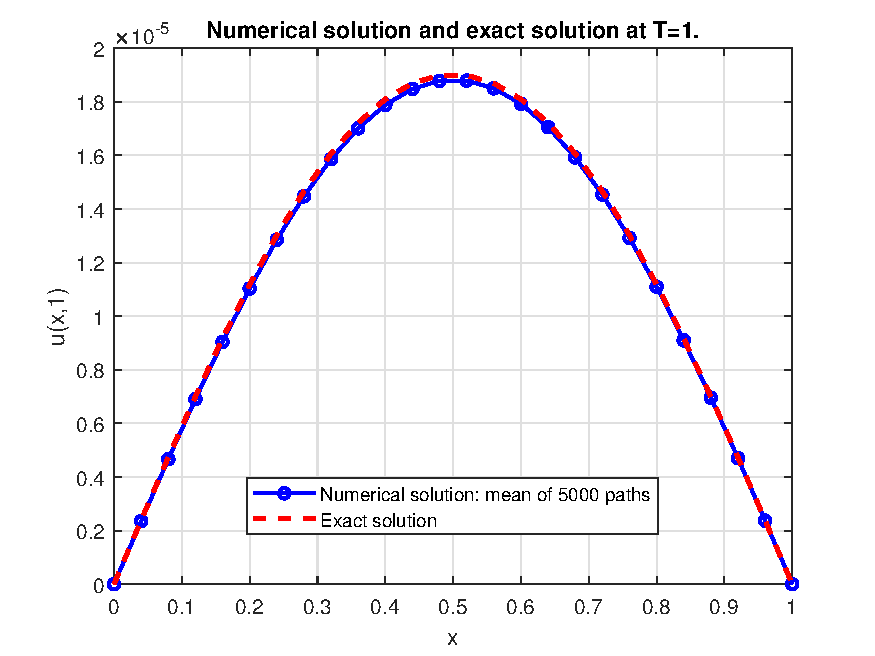
\includegraphics[width=0.48\linewidth,height=0.3\textheight,keepaspectratio]{1-A-eps-converted-to.pdf} & 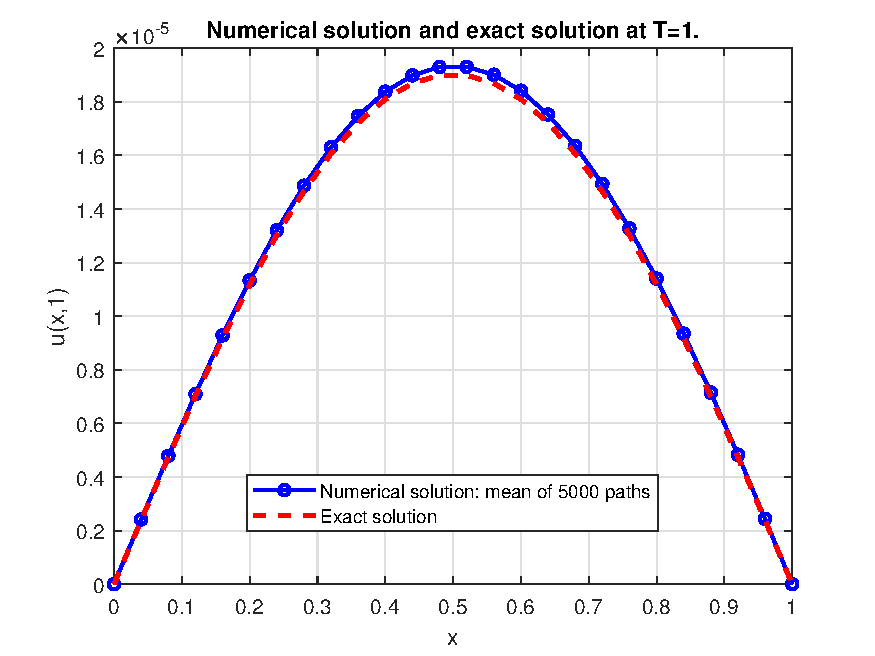
\includegraphics[width=0.48\linewidth,height=0.3\textheight,keepaspectratio]{2-A-eps-converted-to.pdf} \\
	%	\includegraphics[width=0.48\linewidth,height=0.3\textheight,keepaspectratio]{6-eps-converted-to.pdf} & %\includegraphics[width=0.48\linewidth,height=0.3\textheight,keepaspectratio]{7-eps-converted-to.pdf}
	\end{tabular}
	\caption{Comparison of the NSFD scheme with the exact solution for $c=0.5$ and $\Delta x=0.04$, $N=2500$ (left), and for $c=1$ and $\Delta x=0.04$, $N=2000$ (right).
	}
	\label{fig:nsfd-c05-c1}
\end{figure}

\raggedbottom
\begin{figure}[H]
	\centering
	\begin{tabular}{cc}
		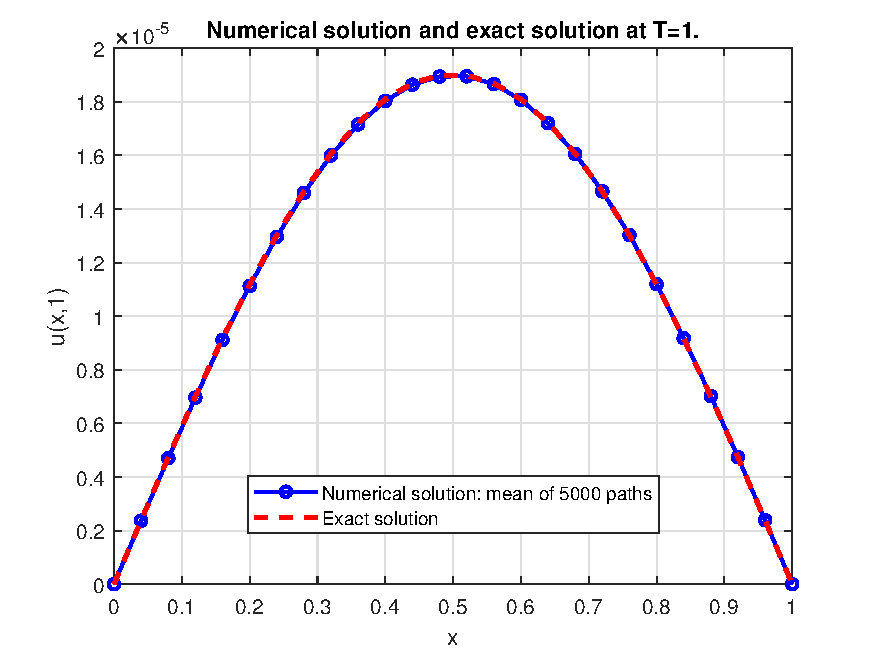
\includegraphics[width=0.48\linewidth,height=0.3\textheight,keepaspectratio]{3-A-eps-converted-to.pdf} & 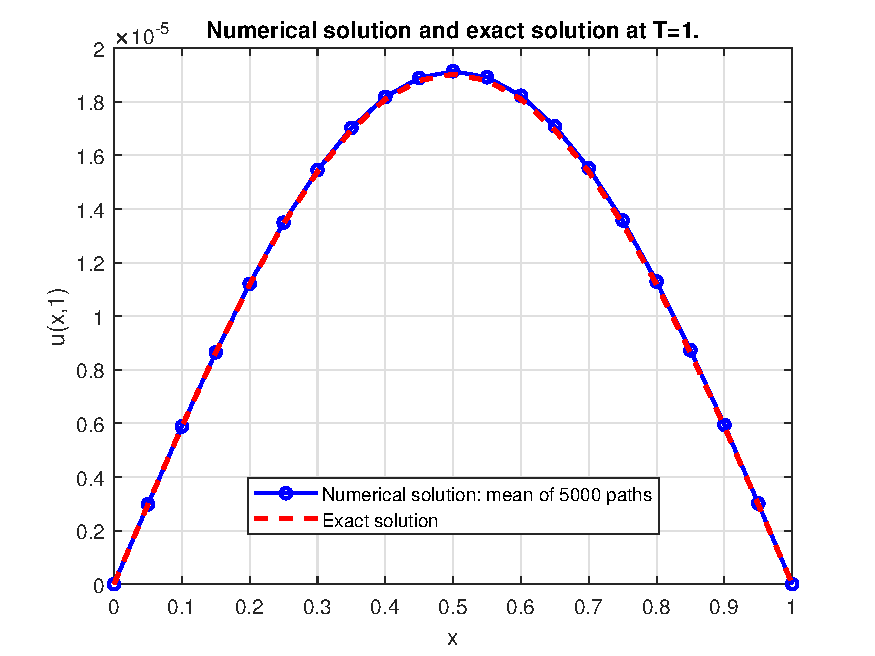
\includegraphics[width=0.48\linewidth,height=0.3\textheight,keepaspectratio]{4-A-eps-converted-to.pdf} \\
		%	\includegraphics[width=0.48\linewidth,height=0.3\textheight,keepaspectratio]{6-eps-converted-to.pdf} & %\includegraphics[width=0.48\linewidth,height=0.3\textheight,keepaspectratio]{7-eps-converted-to.pdf}
	\end{tabular}
	\caption{Comparison of the NSFD scheme with the exact solution for $c=2$ and $\Delta x=0.04$, $N=5000$ (left), and for $c=0.5$ and $\Delta x=0.05$, $N=5000$ (right).
	}
\end{figure}

\raggedbottom
\begin{figure}[H]
	\centering
	\begin{tabular}{cc}
		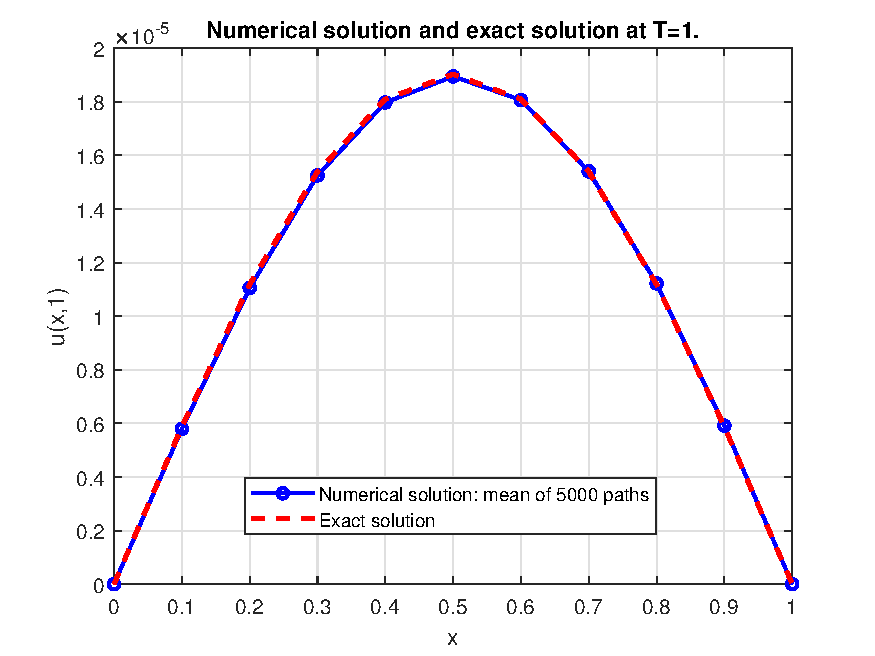
\includegraphics[width=0.48\linewidth,height=0.3\textheight,keepaspectratio]{5-A-eps-converted-to.pdf} & 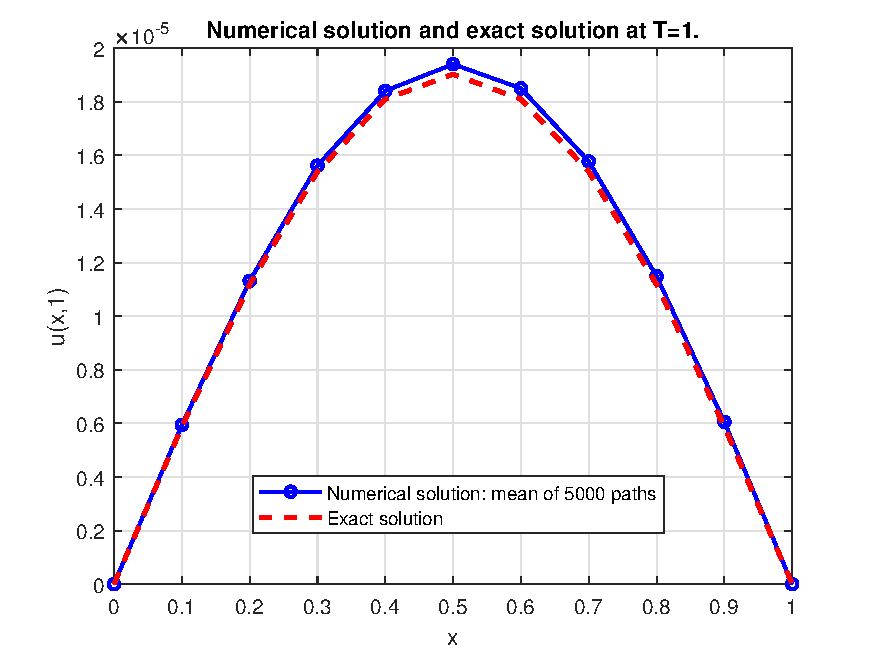
\includegraphics[width=0.48\linewidth,height=0.3\textheight,keepaspectratio]{6-A-eps-converted-to.pdf} \\
		%	\includegraphics[width=0.48\linewidth,height=0.3\textheight,keepaspectratio]{6-eps-converted-to.pdf} & %\includegraphics[width=0.48\linewidth,height=0.3\textheight,keepaspectratio]{7-eps-converted-to.pdf}
	\end{tabular}
	\caption{Comparison of the NSFD scheme with the exact solution for $c=1$ and $\Delta x=0.1$, $N=500$ (left), and for $c=2$ and $\Delta x=0.1$, $N=10000$ (right).
	}
\end{figure}

\raggedbottom


\begin{figure}[H]\label{a4}
	\centering
	\begin{tabular}{cc}
		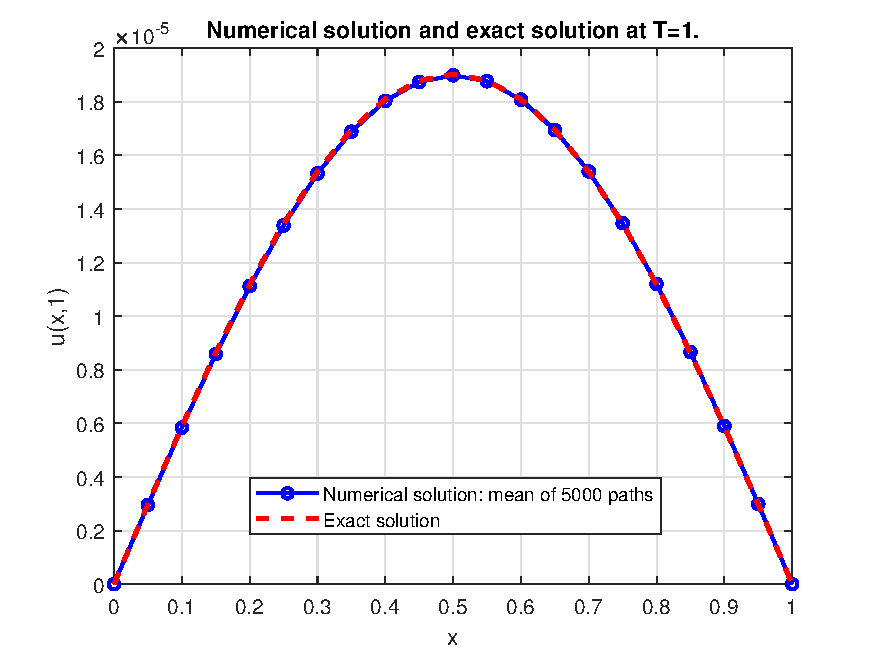
\includegraphics[width=0.48\linewidth,height=0.3\textheight,keepaspectratio]{7-A-eps-converted-to.pdf} & 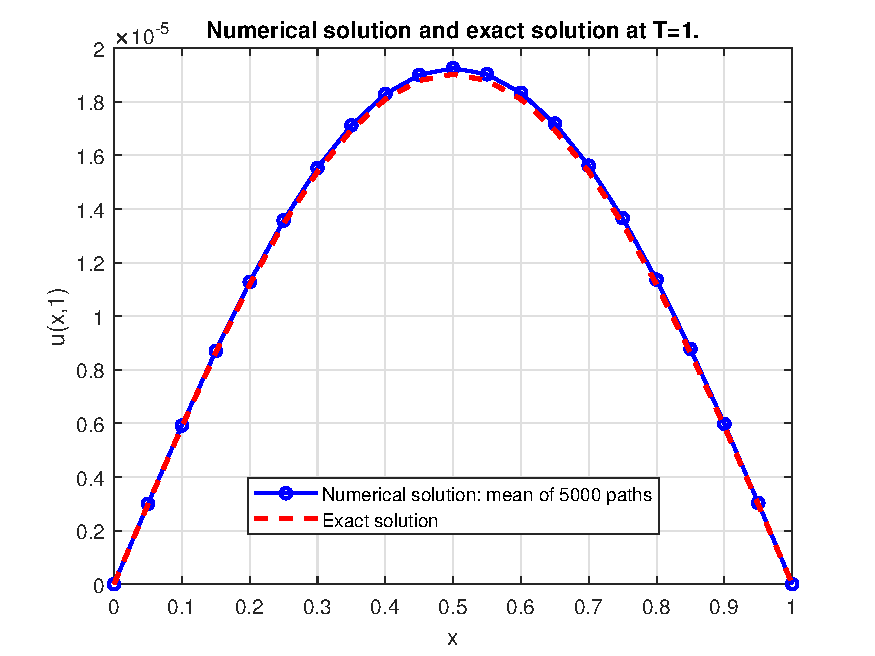
\includegraphics[width=0.48\linewidth,height=0.3\textheight,keepaspectratio]{8-A-eps-converted-to.pdf} \\
		%	\includegraphics[width=0.48\linewidth,height=0.3\textheight,keepaspectratio]{6-eps-converted-to.pdf} & %\includegraphics[width=0.48\linewidth,height=0.3\textheight,keepaspectratio]{7-eps-converted-to.pdf}
	\end{tabular}
	\caption{Comparison of the NSFD scheme with the exact solution for $c=1$ and $\Delta x=0.05$, $N=6000$ (left), and for $c=2$ and $\Delta x=0.05$, $N=15000$ (right).
	}
	\label{fig:nsfd-c05-c2}
\end{figure}

\raggedbottom


\section{Conclusions}
In the present study, an NSFD scheme is 
proposed for the stochastic parabolic partial differential equation. 
The consistency, stability, and convergence of the scheme are 
theoretically established. The numerical study shows that the proposed 
NSFD scheme is a reliable and effective method for solving SPDEs.



\begin{thebibliography}{99}
	\bibitem[Kloeden and Platen (1995)]{Kloeden:Platen:1995} 
	Kloeden P.E. and Platen E. (1995), {\it Numerical solution of stochastic differential equations,} Berlin, Springer.
	
	\bibitem[Roth (2002)]{Roth:2002}
	Roth C. (2002), Difference methods for stochastic partial differential equations, {\it Z. Angew. Math. Mech.} 82, 821-830.
	
	\bibitem[Namjoo and Zibaei (2020)]{Namjoo:Zibaei:2020}
	Namjoo M. and Zibaei S. (2020), A NSFD Scheme for the Solving Fractional-Order Competitive Prey-Predator System, {\it Thai J. Math.} 18, 1933-1945.
	
	\bibitem[Namjoo et al. (2024)]{Namjoo:etal:2024}
	Namjoo M., Aminian M., Mohebbian A., Karami M. and Salmei H. (2024), Upwind Implicit Scheme for the Numerical Solution of Stochastic Advection-Diffusion Partial Differential Equations, {\it Analytical and Numerical Solutions for Nonlinear Equations} 8(2), 138-162.
	
	\bibitem[Karami et al. (2023)]{Karami:etal:2023}
	Karami M., Mohebbian A., Razaghian S., Namjoo M. and Aminian M. (2023), Numerical solutions for a class stochastic partial differential equations, {\it Journal of Mahani Mathematical Research} 13(1), 357-382.
	
	\bibitem[Baleanu et al. (2023)]{Baleanu:etal:2023}
	Baleanu D., Namjoo M., Mohebbian A. and Jajarmi A. (2023), A weighted average finite difference scheme for the numerical solution of stochastic parabolic partial differential equations, {\it CMES-Computer Modeling in Engineering \& Sciences} 135(2).
	
	\bibitem[Namjoo and Mohebbian (2016)]{Namjoo:Mohebbian:2016}
	Namjoo M. and Mohebbian A. (2016), Approximation of stochastic advection diffusion equations with finite difference scheme, {\it Journal of Mathematical Modeling} 4(1), 1-8.
	
	\bibitem[Namjoo and Mohebbian (2019)]{Namjoo:Mohebbian:2019}
	Namjoo M. and Mohebbian A. (2019), Analysis of the stability and convergence of a finite difference approximation for stochastic partial differential equations, {\it Computational Methods for Differential Equations} 7(3), 334-358.
	
	\bibitem[Namjoo et al. (2025)]{Namjoo:etal:2025}
	Namjoo M., Razaghian S., Karami M. and Aminian M. (2025), Nonstandard finite difference schemes for the HIV infection model of CD4+ T-cells, {\it Journal of Difference Equations and Applications} 31(6), 864-891.
	
	\bibitem[Karami et al. (2024)]{Karami:etal:2024}
	Karami M., Razaghian S., Mohebbian A., Namjoo M. and Aminian M. (2024), Analysis of the stability of a nonstandard finite difference scheme for fractional order Lotka–Volterra model, {\it Wavelet Linear Algebra} 11(3), 61-90.
	
	\bibitem[Namjoo and Zibaei (2019)]{Namjoo:Zibaei:2019}
	Namjoo M. and Zibaei S. (2019), Approximation of the Huxley equation with nonstandard finite-difference scheme, {\it Iranian Journal of Numerical Analysis and Optimization} 9(1), 17-35.
	
	\bibitem[Mickens (2020)]{Mickens:2020}
	Mickens R.E. (2020), {\it Nonstandard finite difference schemes: methodology and applications,} World Scientific.
	
	\bibitem[Namjoo et al. (2018)]{Namjoo:etal:2018}
	Namjoo M., Zeinadini M. and Zibaei S. (2018), Nonstandard finite-difference scheme to approximate the generalized Burgers-Fisher equation, {\it Mathematical Methods in the Applied Sciences} 41(17), 8212-8228.
	
	\bibitem[Namjoo and Zibaei (2020)]{Namjoo:Zibaei:2020}
	Namjoo M. and Zibaei S. (2020), A NSFD Scheme for the Solving Fractional-Order Competitive Prey-Predator System, {\it Thai Journal of Mathematics} 18(4), 1933-1945.
	
\end{thebibliography}



\end{document}

